\subsection{Shape Creation}

% SHAPE CREATION AND TRANSFORMATIONS
% for modeling simple buildings
% their translation, scaling, etc.
%\TODO{shape creation}
%\TODO{transformations}

In this section two solutions suitable for conceptual sketching of 3D forms are analyzed.

\subsubsection{SESAME, 2006}

Oh, Stuerzlinger and Danahy \cite{SESAME3D} developed SESAME
(Sketch, Extrude, Sculpt, and Manipulate Easily).
This system focus on providing an interface as powerful and easy as 2D sketching on paper.
Authors defend that a 3D model is more easily understood between users than a regular conceptual design.
It is optimized for modification and allows the creation and editing of volumetric geometry
by extruding 2D contours or sculpting 3D volumes.
It features a simple toolbar interface, allowing the creation of lines,
arcs and free-form curves with constraints.
SESAME also supports automatic grouping of objects, i.e., objects related
between themselves (ex: cup on top of table) affect each other.
User tests conducted comparing SESAME with the modeling package
Autodesk 3D Studio Max have shown that even experienced 3DSM users found
the drawings done with SESAME to be more creative and satisfying.

\begin{figure}[!ht]
	\centering
	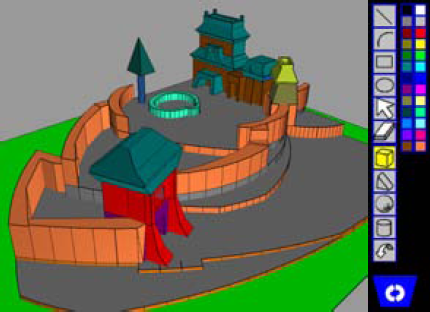
\includegraphics[width=6cm]{gfx/sesame.png}
	\caption{A view of a drawing done in 40 minutes with SESAME}
	\label{FIG-SESAME}
\end{figure}

%\paragraph{Discussion}

This is a promising direction for an urban sketching software to go.
The tests against 3D Studio Max were a bit skewed -- the test should
have been conducted against a system of similar approach, such as Google Sketchup.
The offered interface in SESAME is plain and improper for large screens or collaboration.


\subsubsection{SmartPaper, 2004}

Shesh and Chen \cite{SMARTPAPER} developed SmartPaper, a system designed to support
2D sketching featuring oversketching capabilities, sketch on 3D, 3D transforms and
CSG operations. It employs a non-photorealistic rendering technique to convey the
drawing a sketchy look.

\begin{figure}[!ht]
	\centering
	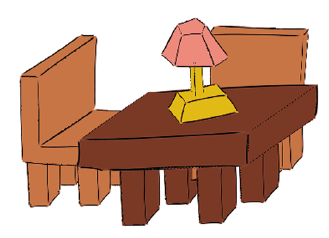
\includegraphics[width=5cm]{gfx/smartpaper.png}
	\caption{Drawing done with SmartPaper}
	\label{FIG-SMARTPAPER}
\end{figure}

\begin{figure}[!ht]
	\centering
	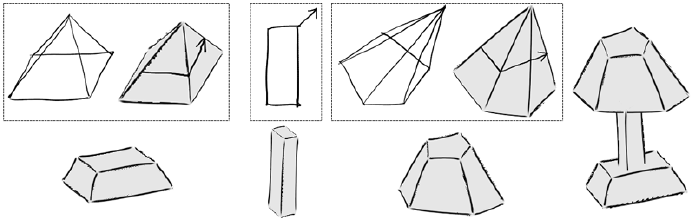
\includegraphics[width=8cm]{gfx/smartpaper2.png}
	\caption{The process of modeling a lamp in SmartPaper}
	\label{FIG-SMARTPAPER2}
\end{figure}

%\paragraph{Discussion}

%The biggest limitation found in SmartPaper is the lack of curved line support.
SmartPaper requires users to draw all object's edges, not only the visible ones.
In the case of extruded objects this is not problematic, since the original face would always have to be drawn anyway.
Another problem is with users having trouble creating perspective drawings.
The resulting geometry appears to be irregular but since the goal is to do
conceptual drawings this is not an issue.

%\TODOL{RELATE TO OUR PROJECT?}
